\appendix
\chapter{Appendix}
If not indicated differently, dimensions and angles specified in the figures
have a tolerance of ±5\%. Unless otherwise noted, all dimensions are in
millimeters (mm). Dimensions and angles defined in the previous chapters may
not be repeated in the figures.

\section{Parallel Parking}
\label{fig_parallel_parking}
\begin{figure}[H]
	\begin{center}
		\centering\includegraphics[width=\textwidth]{graphics/Abb_2_parallel_parking.pdf}
	\end{center}
\end{figure}

\section{Perpendicular Parking}
\begin{figure}[H]
	\label{fig_perpendicular_parking}
	\begin{center}
		\centering\includegraphics[width=\textwidth]{graphics/Abb_3_perpendicular_parking.pdf}
	\end{center}
\end{figure}

\section{Parking Lot}
\label{fig_parking_lot}
\begin{figure}[H]
	\begin{center}
		\centering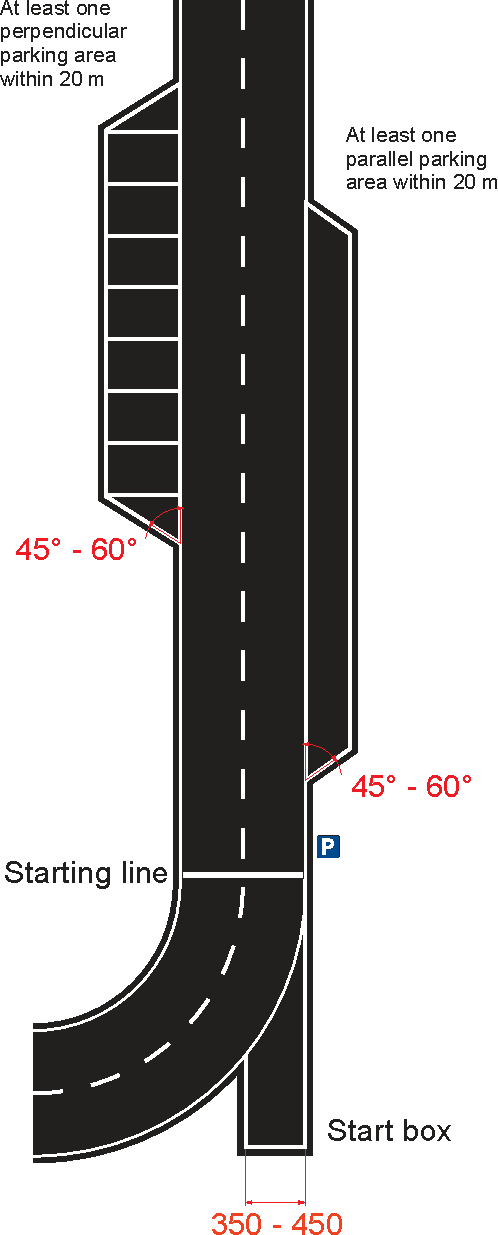
\includegraphics[height=0.9\textheight]{graphics/Abb_1_parking_lot.pdf}
	\end{center}
\end{figure}

\section{Road Layout and Lane Markings}
\label{fig_road_layout}
\begin{figure}[H]
	\begin{center}
		\centering\includegraphics[width=\textwidth]{graphics/Abb_4_road_layout.pdf}
	\end{center}
\end{figure}

\section{Barred Area}
\label{fig_barred_area}
\begin{figure}[H]
	\begin{center}
		\centering\includegraphics[width=\textwidth]{graphics/Abb_8_barred_area.pdf}
	\end{center}
\end{figure}

\section{Intersection of the Rural Road Scenario}
\label{fig_intersection_rural}
\begin{figure}[H]
	\begin{center}
		\centering\includegraphics[scale=0.9]{graphics/Abb_5_intersection.pdf}
	\end{center}
\end{figure}

\subsection{Dynamic Obstacles at Intersections - Give-Way Condition}
\label{fig_intersection_give_way}
\begin{figure}[H]
	\begin{center}
		\centering\includegraphics[scale=0.9]{graphics/Abb_6_intersection_give_way.pdf}
	\end{center}
\end{figure}

\section{Speed Limit Zone}
\label{fig_speed_limit_zone}
\begin{figure}[H]
	\begin{center}
		\centering\includegraphics[height=0.9\textheight]{graphics/Abb_7_speed_limit_zone.pdf}
	\end{center}
\end{figure}

\section{Crosswalk}
\label{fig_crosswalk}
\begin{figure}[H]
	\begin{center}
		\centering\includegraphics[height=0.9\textheight]{graphics/Abb_9_crosswalk.pdf}
	\end{center}
\end{figure}
\newpage

% \section{Pedestrian Island}
% \begin{figure}[H]
% 	\begin{center}
% 		\centering\includegraphics[]{graphics/Abb_10_pedestrian_island.pdf}
% 	\end{center}
% \end{figure}
% \newpage

% \subsection{Pedestrian Island with Crosswalk}
% \begin{figure}[H]
% 	\begin{center}
% 		\centering\includegraphics[]{graphics/Abb_11_pedestrian_island_crosswalk.pdf}
% 	\end{center}
% \end{figure}

\section{Additional Intersections of the Suburban Scenario}
\label{additional_intersections}

\subsection{Intersection with Give-Way Lines}
\label{fig_intersection_give_way_lines}
\begin{figure}[H]
	\begin{center}
		\centering\includegraphics[scale=0.9]{graphics/Abb_12_intersection_give_way_lines.pdf}
	\end{center}
\end{figure}

\vspace{-1em}

\subsection{Intersection with Priority to Right}
\label{fig_intersection_priority}
\begin{figure}[H]
	\begin{center}
		\centering\includegraphics[scale=0.9]{graphics/Abb_13_intersection_priority.pdf}
	\end{center}
\end{figure}

\subsection{Intersection with Mandatory Turn}
\label{fig_intersection_mandatory}
\subsubsection{Mandatory Crossing Direction - Stop Condition}
\begin{figure}[H]
	\begin{center}
		\centering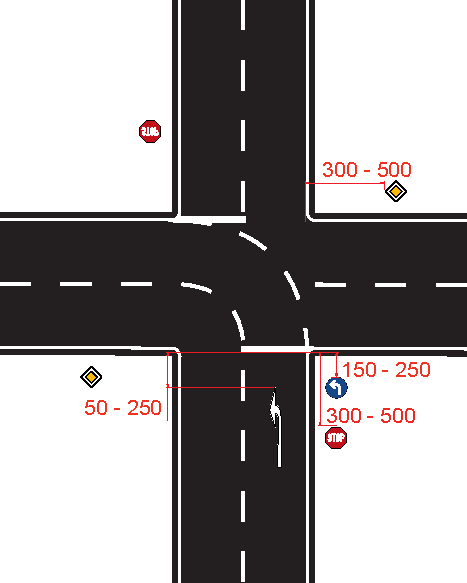
\includegraphics[scale=0.9]{graphics/Abb_14_mandatory_stop.pdf}
	\end{center}
\end{figure}

\vspace{-1em}

\subsubsection{Mandatory Crossing Direction - Give-Way Condition}
\begin{figure}[H]
	\begin{center}
		\centering\includegraphics[scale=0.9]{graphics/Abb_15_mandatory_give_way.pdf}
	\end{center}
\end{figure}

\subsubsection{Mandatory Crossing Direction - Right of Way Condition}
\begin{figure}[H]
	\begin{center}
		\centering\includegraphics[scale=0.9]{graphics/Abb_16_mandatory_right_of_way.pdf}
	\end{center}
\end{figure}

\vspace{-1em}

\section{Road Markings}
\label{fig_road_markings}
\begin{figure}[H]
	\begin{center}
		\centering\includegraphics[width=\textwidth]{graphics/Abb_17_road_markings.pdf}
	\end{center}
\end{figure}

\section{Traffic Signs}
\label{fig_traffic_signs}

The traffic signs are defined according to StVO (Legal definition of traffic
rules) and are applied as described there, except otherwise defined in this
document. Additional information about the dimensions can be scaled based on
this source.

Traffic signs might appear in their mirrored version as well, e.g. turning
symbols can indicate right or left turns.

\begin{figure}[H]
	\begin{center}
		\centering\includegraphics[]{graphics/Abb_18_traffic_signs.pdf}
	\end{center}
\end{figure}

\subsection{Positioning of Traffic Signs}
\begin{figure}[H]
	\begin{center}
		\centering\includegraphics[]{graphics/Abb_19_positioning_of_traffic_signs.pdf}
	\end{center}
\end{figure}

\begin{highlight}[green]
\section{Landmarks}
\label{fig_landmarks}

Landmarks are additional "traffic signs" serving as navigation points for the
vehicle. Each landmark will depict a QR code with a unique identifier.

\begin{figure}[H]
	\begin{center}
		\centering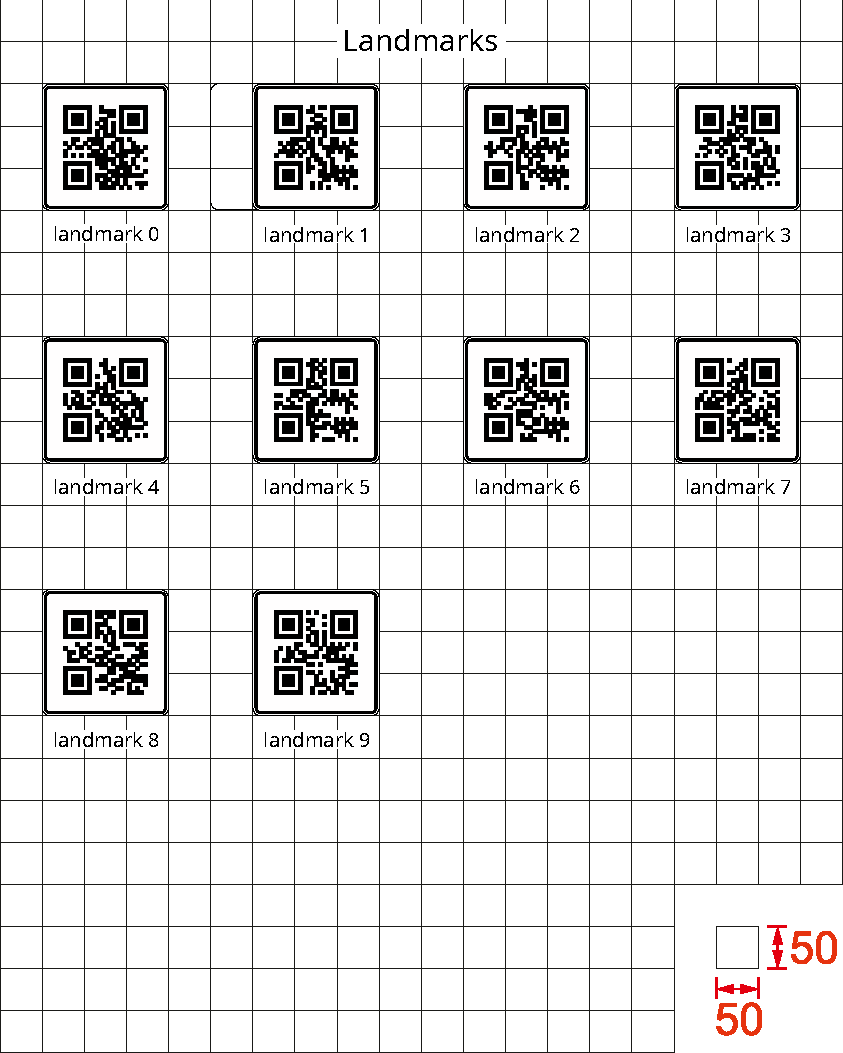
\includegraphics[]{graphics/Abb_24_landmarks.pdf}
	\end{center}
\end{figure}
\end{highlight}

\section{Dimensions of Obstacles}
\subsection{Static and Dynamic Obstacles on the Track}
\label{fig_obstacle_dimensions}
\begin{figure}[H]
	\begin{center}
		\centering\includegraphics[]{graphics/Abb_20_obstacles.pdf}
	\end{center}
\end{figure}

\subsection{Pedestrians}
\label{fig_pedestrians}
\begin{figure}[H]
	\begin{center}
		\centering\includegraphics[width=\textwidth]{graphics/Abb_21_pedestrians.pdf}
	\end{center}
\end{figure}

\section{Markings of the Start Box Gate}
\label{fig_start_box_markings}
\begin{figure}[H]
	\begin{center}
		\centering\includegraphics[width=\textwidth]{graphics/Abb_23_start_box_markings.pdf}
	\end{center}
\end{figure}

\section{Example Circuit}
\label{fig_example_circuit}
\vspace*{2cm}
\begin{figure}[H]
	\begin{center}
		\centering\includegraphics[width=\textwidth]{graphics/Abb_22_example_circuit.pdf}
	\end{center}
\end{figure}

